% ===============================================================
% APRESENTAÇÃO (BEAMER) - TCC2 - SENAC SANTO AMARO
% ===============================================================
% Baseada no modelo apresentacao_tcc2.tex do repositório
% afonsolelis/template_tcc_senac.
%
% 26 slides de conteúdo, mais capa, roteiro e encerramento.
%
% COMO COMPILAR (na raiz do repositório):
%   pdflatex apresentacao_tcc2.tex
%   pdflatex apresentacao_tcc2.tex   (2x para fixar índice/numeração)
% ===============================================================

\documentclass[
    aspectratio=169,
    12pt,
    brazil,
    xcolor=table
]{beamer}

% ---------------------------------------------------------------
% PACOTES
% ---------------------------------------------------------------
\usepackage{lmodern}
\usepackage[T1]{fontenc}
\usepackage[utf8]{inputenc}
\usepackage[brazil]{babel}
\usepackage{graphicx}
\usepackage{booktabs}
\usepackage{tikz}
\usepackage{appendixnumberbeamer}

% ---------------------------------------------------------------
% TEMA E CORES
% ---------------------------------------------------------------
\usetheme{default}
\useinnertheme{circles}
\setbeamertemplate{navigation symbols}{}
\setbeamersize{text margin left=0.7cm,text margin right=0.7cm}

\definecolor{senacblue}{RGB}{0,51,102}
\definecolor{senacorange}{RGB}{243,146,0}

\setbeamercolor{structure}{fg=senacblue}
\setbeamercolor{frametitle}{fg=white,bg=senacblue}
\setbeamercolor{title}{fg=senacblue}
\setbeamercolor{section in toc}{fg=senacblue}
\setbeamercolor{itemize item}{fg=senacorange}
\setbeamercolor{itemize subitem}{fg=senacorange}
\setbeamerfont{frametitle}{series=\bfseries}
\setbeamertemplate{frametitle}[default][left]

\setbeamertemplate{footline}{%
  \leavevmode%
  \hbox{%
    \begin{beamercolorbox}[wd=.34\paperwidth,ht=2.4ex,dp=1ex,leftskip=1em]{author in head/foot}%
      \usebeamerfont{author in head/foot}\insertshortauthor
    \end{beamercolorbox}%
    \begin{beamercolorbox}[wd=.5\paperwidth,ht=2.4ex,dp=1ex,center]{title in head/foot}%
      \usebeamerfont{title in head/foot}\insertshorttitle
    \end{beamercolorbox}%
    \begin{beamercolorbox}[wd=.16\paperwidth,ht=2.4ex,dp=1ex,rightskip=1em]{title in head/foot}%
      \usebeamerfont{title in head/foot}\hfill\insertframenumber/\inserttotalframenumber
    \end{beamercolorbox}%
  }\vskip0pt%
}
\setbeamercolor{author in head/foot}{bg=senacblue,fg=white}
\setbeamercolor{title in head/foot}{bg=senacblue!85,fg=white}

% ---------------------------------------------------------------
% LOGO DO SENAC (grande na capa, pequena no canto dos demais slides)
% ---------------------------------------------------------------
\newcommand{\logosenacgrande}{%
  \IfFileExists{assets/logo-senac.png}{%
    
\includegraphics[height=2.6cm]{assets/logo-senac.png}%
  }{%
    \begin{tikzpicture}
      \node[draw=senacblue,line width=1pt,rounded corners,
            minimum width=4.5cm,minimum height=2.4cm,align=center,
            fill=senacblue!5]
        {\bfseries\color{senacblue}\Large SENAC\\[2pt]
         \normalsize Santo Amaro};
    \end{tikzpicture}%
  }%
}

\newcommand{\logosenacpequena}{%
  \IfFileExists{assets/logo-senac.png}{%
    
\includegraphics[height=0.8cm]{assets/logo-senac.png}%
  }{%
    \fbox{\scriptsize\bfseries\color{senacblue}SENAC}%
  }%
}

\addtobeamertemplate{frametitle}{}{%
  \begin{tikzpicture}[remember picture,overlay]
    \node[anchor=north east,fill=white,rounded corners=2pt,inner sep=3pt]
      at ([xshift=-6pt,yshift=-5pt]current page.north east) {\logosenacpequena};
  \end{tikzpicture}%
}

% Fonte de imagens de terceiros e notas de rodapé dos slides
\newcommand{\fontefig}[1]{\par\vspace{2pt}{\centering\tiny Fonte: #1\par}}
\newcommand{\nota}[1]{\par\vspace{3pt}{\scriptsize #1\par}}
\newcommand{\destaque}[1]{{\color{senacblue}\bfseries #1}}

% ---------------------------------------------------------------
% DADOS DA APRESENTAÇÃO
% ---------------------------------------------------------------
\title[Inferência SepConv em C++: eficiência e VRAM]{Análise Experimental da Inferência SepConv em C++ com Ênfase em Eficiência Computacional e Uso de VRAM}
\subtitle{Apresentação final, TCC2}
\author[Pedro Henrique Gomes]{Pedro Henrique Gomes}
\institute[SENAC Santo Amaro]{%
  SENAC, Unidade Santo Amaro\\
  Bacharelado em Ciência da Computação\\
  \footnotesize Orientador: Prof. Afonso Brandão}
\date{São Paulo, 2026}

% ===============================================================
\begin{document}

% ---------------------------------------------------------------
% CAPA
% ---------------------------------------------------------------
{
\setbeamertemplate{footline}{}
\begin{frame}[plain]
  \centering
  \vspace{0.1cm}
  \logosenacgrande

  \vspace{0.3cm}
  {\usebeamerfont{title}\usebeamercolor[fg]{title}\bfseries\large\inserttitle\par}
  \vspace{0.15cm}
  {\normalsize\insertsubtitle\par}

  \vspace{0.3cm}
  {\small\insertauthor\par}
  \vspace{0.1cm}
  {\footnotesize\insertinstitute\par}

  \vfill
  {\footnotesize\insertdate\par}
\end{frame}
}

% ---------------------------------------------------------------
% ROTEIRO
% ---------------------------------------------------------------
\begin{frame}{Roteiro da apresentação}
  \tableofcontents
\end{frame}

% ===============================================================
\section{Introdução e problema}
% ===============================================================
\begin{frame}{Contexto: criar o quadro do meio}
  \centering
  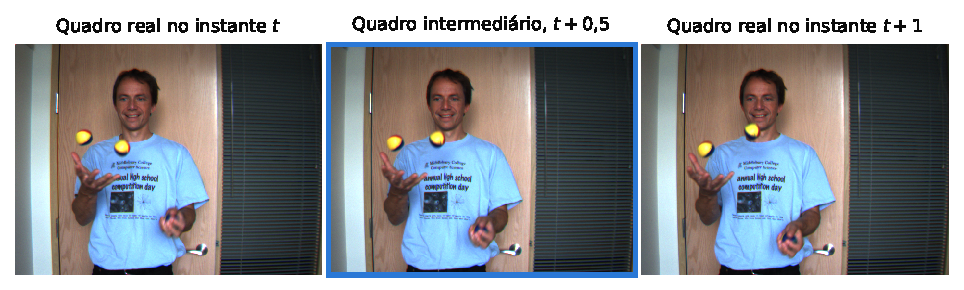
\includegraphics[width=\textwidth]{imagens/vfi_sequencia.pdf}
  \fontefig{elaborado pelo autor, com a sequência Beanbags do Middlebury (BAKER et al., 2011).}
  \vspace{4pt}
  \raggedright\small
  \begin{itemize}
    \item Muitos vídeos têm 24 ou 30 FPS, e as telas atualizam de 60 Hz a 144 Hz.
    \item A interpolação de quadros (VFI) sintetiza as imagens que faltam entre dois quadros.
  \end{itemize}
\end{frame}

\begin{frame}{Repetir, misturar ou interpolar?}
  \centering
  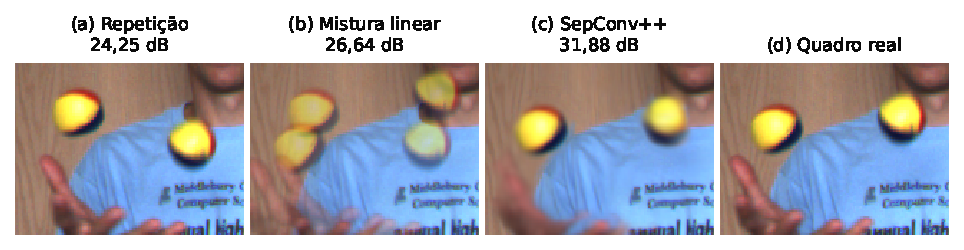
\includegraphics[width=\textwidth]{imagens/vfi_metodos.pdf}
  \fontefig{elaborado pelo autor, com a sequência Beanbags do Middlebury (BAKER et al., 2011).}
  \vspace{4pt}
  \raggedright\small
  \begin{itemize}
    \item \textbf{Repetição:} a bola fica na posição antiga.
    \item \textbf{Mistura:} surgem duas bolas semitransparentes (\textit{ghosting}).
    \item \textbf{SepConv++:} uma bola só, perto da posição real, com algum borramento.
  \end{itemize}
\end{frame}

\begin{frame}{Filtros adaptativos: um filtro por pixel}
  \begin{columns}[T]
    \begin{column}{0.62\textwidth}
      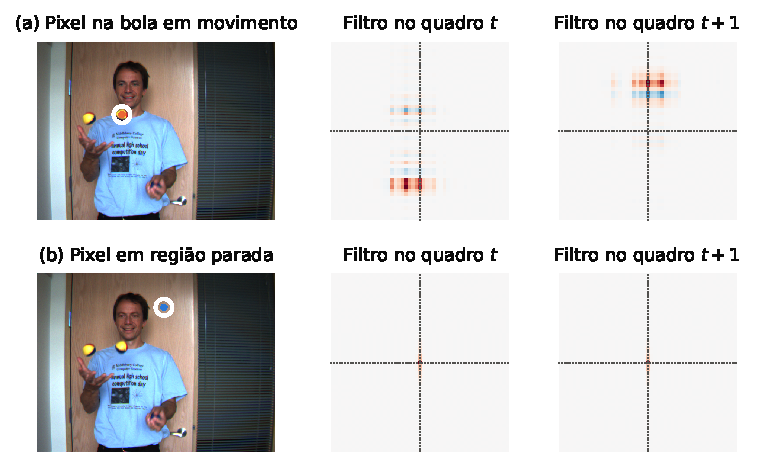
\includegraphics[width=\linewidth]{imagens/filtro_adaptativo.pdf}
      \fontefig{elaborado pelo autor, com a sequência Beanbags (BAKER et al., 2011).}
    \end{column}
    \begin{column}{0.36\textwidth}
      \small
      \begin{itemize}
        \item A rede não gera o pixel: ela gera os pesos para sintetizá-lo.
        \item \textbf{Parado:} peso no centro do filtro.
        \item \textbf{Bola:} peso em $(-4,+16)$ no quadro $t$ e em $(0,-14)$ em $t+1$.
        \item O movimento fica implícito nos pesos, sem fluxo óptico.
      \end{itemize}
    \end{column}
  \end{columns}
\end{frame}

\begin{frame}{Separabilidade: menos memória nos filtros}
  \begin{columns}[T]
    \begin{column}{0.5\textwidth}
      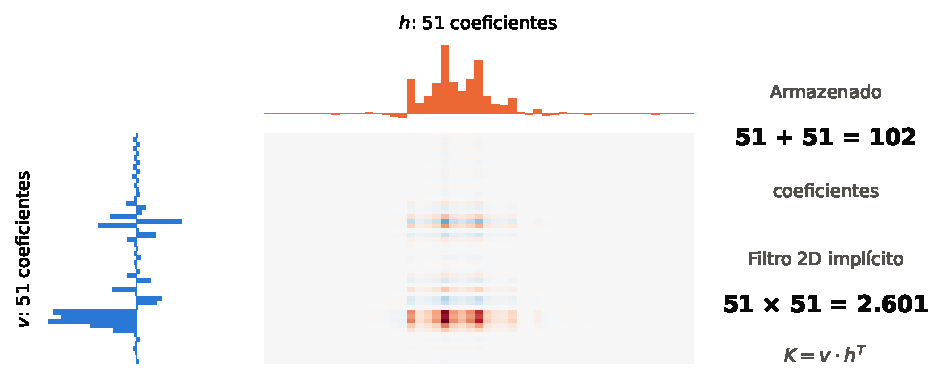
\includegraphics[width=\linewidth]{imagens/separabilidade.pdf}
      \vspace{2pt}
      \small
      \begin{itemize}
        \item Dois vetores 1D em vez de uma matriz 2D.
        \item 102 coeficientes por pixel, contra 2.601.
        \item A síntese continua com $N^2$ multiplicações: o ganho é de memória.
      \end{itemize}
    \end{column}
    \begin{column}{0.5\textwidth}
      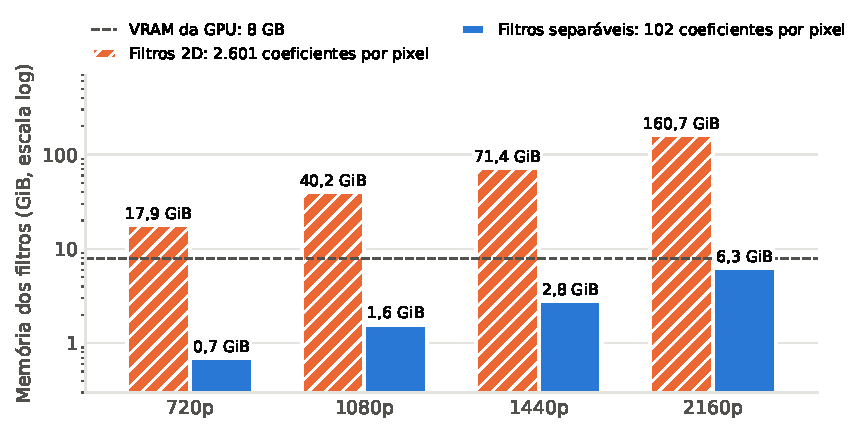
\includegraphics[width=\linewidth]{imagens/memoria_filtros.pdf}
      \vspace{2pt}
      \small
      \begin{center}
        Em 1080p: \destaque{1,6 GB contra 40 GB}\\
        É o que torna o modelo viável em 8 GB.
      \end{center}
    \end{column}
  \end{columns}
\end{frame}

\begin{frame}{O gargalo: memória da GPU}
  \centering
  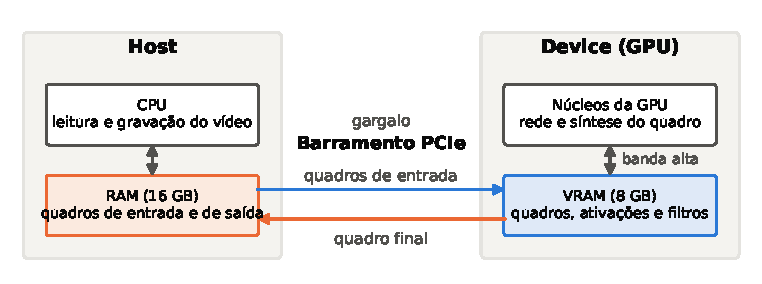
\includegraphics[width=0.92\textwidth]{imagens/host_device.pdf}
  \vspace{4pt}
  \raggedright\small
  \begin{itemize}
    \item A VRAM é um limite físico: quando acaba, o \textit{driver} usa a RAM e o tempo dispara.
    \item O barramento PCIe é mais lento que a memória interna da GPU.
    \item GPUs de 8 GB representam cerca de 26\% das configurações na pesquisa da Steam.
  \end{itemize}
\end{frame}

\begin{frame}{Trabalhos correlatos}
  \centering
  \footnotesize
  \renewcommand{\arraystretch}{1.25}
  \begin{tabular}{p{2.9cm}p{5.1cm}p{5.1cm}}
    \toprule
    \textbf{Trabalho} & \textbf{Estratégia} & \textbf{Limitação ou diferencial} \\
    \midrule
    Teed e Deng (2020) & RAFT: fluxo óptico recorrente, com atualização iterativa & Alto custo computacional e de VRAM \\
    Niklaus et al. (2021) & SepConv++: convoluções adaptativas separáveis refinadas & Execução dependente do PyTorch \\
    Han et al. (2024) & Movimento multiescala com pirâmide hierárquica & Maior complexidade da arquitetura \\
    \rowcolor{senacblue!15}
    \textbf{Este trabalho} & \textbf{Inferência nativa: ONNX Runtime e \textit{kernel} CUDA} & \textbf{Mede latência e VRAM em GPU de 8 GB} \\
    \bottomrule
  \end{tabular}
  \vspace{8pt}

  \small O modelo é o mesmo do SepConv++: o que muda é como a inferência é executada.
\end{frame}

\begin{frame}{Problema e pergunta de pesquisa}
  \begin{itemize}
    \item Modelos de VFI dependem de \textit{frameworks} de alto nível e exigem muita VRAM.
    \item Isso dificulta a execução em computadores com GPUs de consumo.
  \end{itemize}
  \vspace{6pt}
  \begin{block}{Pergunta de pesquisa}
    Em que medida um motor de inferência nativo em C++ e CUDA para o modelo SepConv reduz a latência e o consumo de VRAM em GPUs de consumo de 8 GB, mantendo a fidelidade visual da implementação original?
  \end{block}
\end{frame}

% ===============================================================
\section{Objetivos e método}
% ===============================================================
\begin{frame}{Objetivos}
  \small
  \begin{block}{Objetivo geral}
    Determinar em que medida um motor nativo em C++ e CUDA reduz a latência e o pico de VRAM em uma GPU de 8 GB, em relação à implementação original, mantendo a fidelidade visual.
  \end{block}
  \vspace{2pt}
  \textbf{Objetivos específicos:}
  \begin{enumerate}
    \item Verificar a equivalência numérica entre as saídas do motor e da original;
    \item Quantificar a diferença de latência, de 720p a 2160p (H1);
    \item Determinar o efeito sobre o pico de VRAM e onde a memória se esgota (H2);
    \item Verificar a fidelidade no vídeo de teste e em conjuntos de referência (H3);
    \item Identificar as fontes do consumo e medir alocador, precisão e blocos;
    \item Separar o efeito da forma de execução do efeito da precisão.
  \end{enumerate}
\end{frame}

\begin{frame}{Hipótese e critérios de validação}
  Um motor nativo reduz a latência e o pico de VRAM, sem degradar a fidelidade.
  \vspace{8pt}

  \centering
  \small
  \renewcommand{\arraystretch}{1.3}
  \begin{tabular}{lp{10.4cm}}
    \toprule
    \textbf{Critério} & \textbf{Condição, em cada resolução} \\
    \midrule
    \textbf{H1: latência} & Redução de pelo menos 10\%, com teste $t$ de Welch unilateral ($\alpha = 0{,}05$) \\
    \textbf{H2: VRAM} & Pico de no máximo 90\% do pico da original, sem saturar a GPU \\
    \textbf{H3: fidelidade} & Diferença média de até 0,1 dB de PSNR, 0,001 de SSIM e 0,5 de VMAF \\
    \bottomrule
  \end{tabular}
  \vspace{8pt}

  \raggedright
  Os critérios valem para 720p e 1080p. As resoluções 1440p e 2160p mostram o que acontece quando a VRAM se esgota.
\end{frame}

\begin{frame}{Método de pesquisa e cenário de testes}
  \footnotesize
  \begin{columns}[T]
    \begin{column}{0.5\textwidth}
      \textbf{Estudo experimental comparativo}
      \begin{itemize}
        \item \textbf{Variáveis manipuladas:} implementação, resolução e, depois, versão do motor e precisão.
        \item \textbf{Variáveis medidas:} tempo por quadro, pico de VRAM, PSNR, SSIM e VMAF.
        \item \textbf{Referência:} código original em Python/PyTorch.
        \item \textbf{Ambiente:} RTX 4060 Ti de 8 GB, i5-12400F, 16 GB de RAM, Windows 11.
      \end{itemize}
    \end{column}
    \begin{column}{0.5\textwidth}
      \textbf{Protocolo das baterias}
      \begin{itemize}
        \item Trecho de 61 quadros do trailer do GTA VI, em FFV1, de 720p a 2160p.
        \item Vídeo de 15 para 30 FPS: os quadros sintetizados são comparados aos reais.
        \item 27 medições após 3 de aquecimento (em 2160p, 3 após 1).
        \item VRAM pela NVML; a partir da 3ª bateria, a cada 1 ms.
        \item Qualidade também no Middlebury e no Vimeo-90K.
      \end{itemize}
    \end{column}
  \end{columns}
\end{frame}

% ===============================================================
\section{Desenvolvimento}
% ===============================================================
\begin{frame}{Solução desenvolvida: três versões}
  \centering
  \small
  \renewcommand{\arraystretch}{1.35}
  \begin{tabular}{lp{5.2cm}p{6.4cm}}
    \toprule
    \textbf{Versão} & \textbf{O que mudou} & \textbf{Pergunta respondida} \\
    \midrule
    \textbf{v1} & OpenCV, ONNX Runtime e \textit{kernel} CUDA próprio, com o quadro inteiro & Só trocar a forma de execução já traz ganho? \\
    \textbf{v2} & Processamento em blocos, com margem de 96 pixels & O pico de memória pode deixar de depender da resolução? \\
    \textbf{v3} & Alocador ajustado e meia precisão (FP16) & De onde vinha o consumo excedente? \\
    \bottomrule
  \end{tabular}
  \vspace{10pt}

  \raggedright
  Cada versão nasceu do resultado da anterior e foi medida em uma bateria própria. Uma quarta bateria comparou as quatro combinações de implementação e precisão.
\end{frame}

\begin{frame}{Arquitetura do motor}
  \centering
  \begin{tikzpicture}[
      x=1cm,y=1cm,
      etapa/.style={draw=senacblue,rounded corners=2pt,minimum width=4.1cm,minimum height=1.25cm,align=center,font=\footnotesize,fill=gray!12},
      vram/.style={etapa,fill=senacblue!15},
      seta/.style={->,thick,senacblue}]
    \node[etapa] (e1) at (0,2.1) {\textbf{1. Leitura (OpenCV)}\\quadros \textit{uint8} na RAM};
    \node[vram]  (e2) at (4.7,2.1) {\textbf{2. Host $\rightarrow$ Device}\\cópia dos quadros via PCIe};
    \node[vram]  (e3) at (9.4,2.1) {\textbf{3. Pré-processamento}\\\textit{kernel} CUDA: \textit{float} planar};
    \node[vram]  (e4) at (9.4,0) {\textbf{4. Inferência}\\ONNX Runtime: 4 tensores 1D};
    \node[vram]  (e5) at (4.7,0) {\textbf{5. Convolução separável}\\\textit{kernel} CUDA próprio};
    \node[etapa] (e6) at (0,0) {\textbf{6. Device $\rightarrow$ Host}\\só o quadro final, e gravação};
    \draw[seta] (e1) -- (e2);
    \draw[seta] (e2) -- (e3);
    \draw[seta] (e3) -- (e4);
    \draw[seta] (e4) -- (e5);
    \draw[seta] (e5) -- (e6);
  \end{tikzpicture}
  \vspace{8pt}

  \raggedright\small
  \begin{itemize}
    \item Em azul, os estágios na VRAM: os dados só saem da GPU no quadro final.
    \item \textit{I/O binding}: entradas e saídas do grafo apontam para \textit{buffers} já alocados na VRAM.
  \end{itemize}
\end{frame}

\begin{frame}{Construção: exportação e síntese}
  \small
  \textbf{Correção da exportação ONNX}
  \begin{itemize}
    \item A primeira exportação só funcionava na resolução em que foi gerada.
    \item Uma condição em Python ficava fixa no grafo; foi trocada por um fatiamento válido para qualquer resolução com dimensões pares.
  \end{itemize}
  \vspace{4pt}
  \textbf{\textit{Kernel} de síntese}
  \begin{itemize}
    \item Cada \textit{thread} calcula um pixel, combinando os filtros 1D e os dois quadros.
    \item Os 51 coeficientes horizontais são lidos uma vez e reutilizados nas 51 linhas.
  \end{itemize}
  \vspace{4pt}
  \begin{block}{Equivalência com a original}
    93,67 dB de PSNR entre as saídas: 0,003\% dos valores diferem, sempre em 1 nível.
  \end{block}
\end{frame}

\begin{frame}{v2: processamento em blocos}
  \begin{columns}[T]
    \begin{column}{0.54\textwidth}
      \begin{tikzpicture}[scale=0.58, every node/.style={font=\scriptsize}]
        \draw[step=2, gray!50] (0,0) grid (12,6);
        \draw[thick] (0,0) rectangle (12,6);
        \fill[blue!8] (3.4,0.6) rectangle (8.6,5.4);
        \draw[blue!70, dashed, thick] (3.4,0.6) rectangle (8.6,5.4);
        \fill[blue!30] (4,2) rectangle (6,4);
        \draw[blue!80!black, thick] (4,2) rectangle (6,4);
        \node[align=center] at (5,3) {miolo\\$T \times T$};
        \draw[<->] (6,3.3) -- (8.6,3.3) node[midway, above] {$M$};
      \end{tikzpicture}
      \nota{Tracejado: recorte enviado à rede (bloco + margem $M$). Só o miolo é aproveitado.}
    \end{column}
    \begin{column}{0.44\textwidth}
      \small
      \begin{itemize}
        \item Filtros e ativações passam a ter o tamanho do bloco.
        \item \textbf{Normalização global}, igual para todos os blocos.
        \item Recortes em \textbf{múltiplos de 16}, por causa da rede.
        \item \textbf{Margem de 96 pixels}: sem ela, erro de até 98 níveis; com ela, 1 nível em menos de 0,002\% dos pixels.
      \end{itemize}
    \end{column}
  \end{columns}
\end{frame}

\begin{frame}{v3: alocador e meia precisão}
  \begin{columns}[T]
    \begin{column}{0.56\textwidth}
      \footnotesize
      \textbf{Alocador, em 1080p (quadro inteiro)}\\[3pt]
      \setlength{\tabcolsep}{4pt}
      \begin{tabular}{lrr}
        \toprule
        \textbf{Configuração} & \textbf{ms} & \textbf{MiB} \\
        \midrule
        Anterior & 307,3 & 6.646 \\
        Sem padrão de memória & 305,7 & 4.743 \\
        Arena liberada a cada execução & 363,2 & 4.743 \\
        \rowcolor{senacblue!15}
        \textbf{Sem padrão, arena em pot. de 2} & \textbf{306,2} & \textbf{4.885} \\
        \bottomrule
      \end{tabular}
      \nota{Desativar o padrão de memória: $-29\%$ de pico, sem custo de tempo. A combinação em destaque foi a adotada porque tem a menor memória sem custo de tempo nos blocos.}
    \end{column}
    \begin{column}{0.42\textwidth}
      \footnotesize
      \textbf{Meia precisão (FP16)}
      \begin{itemize}
        \item Cada número ocupa 16 bits, em vez de 32.
        \item Rede e filtros em FP16: filtros de 1,6 GB para 0,8 GB em 1080p.
        \item Entradas, média e desvio, e acumulação da síntese seguem em FP32.
        \item Diferença de no máximo 1 nível, em cerca de 0,13\% dos pixels.
      \end{itemize}
    \end{column}
  \end{columns}
\end{frame}

% ===============================================================
\section{Resultados e análise}
% ===============================================================
\begin{frame}{v1: latência}
  \begin{columns}[T]
    \begin{column}{0.62\textwidth}
      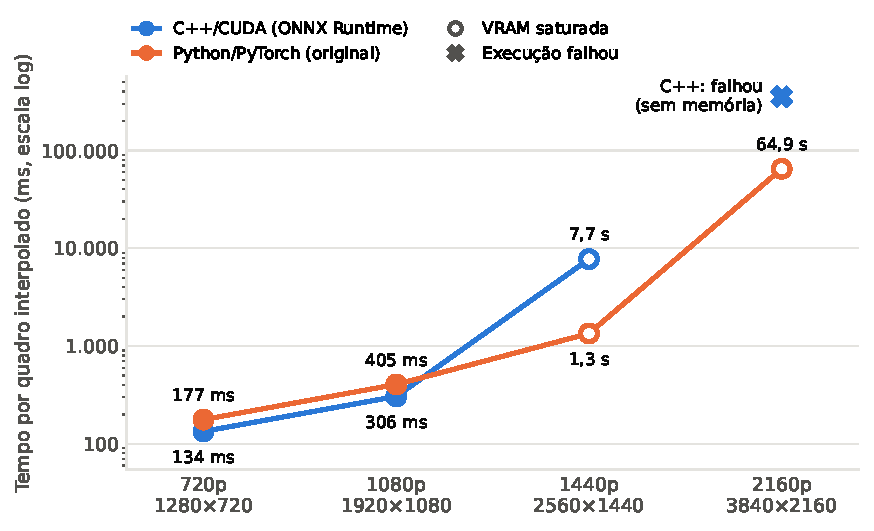
\includegraphics[width=\linewidth,height=6cm,keepaspectratio]{imagens/latencia.pdf}
    \end{column}
    \begin{column}{0.36\textwidth}
      \small
      \begin{itemize}
        \item \destaque{Cerca de 24\% mais rápido} em 720p e 1080p.
        \item 1080p: 305,5 ms contra 404,9 ms.
        \item H1 atendido, com $p < 0{,}001$.
        \item A partir de 1440p, a VRAM se esgota: 7,7 s contra 1,3 s.
        \item Em 2160p, o motor falha.
      \end{itemize}
    \end{column}
  \end{columns}
\end{frame}

\begin{frame}{v1: consumo de VRAM}
  \begin{columns}[T]
    \begin{column}{0.62\textwidth}
      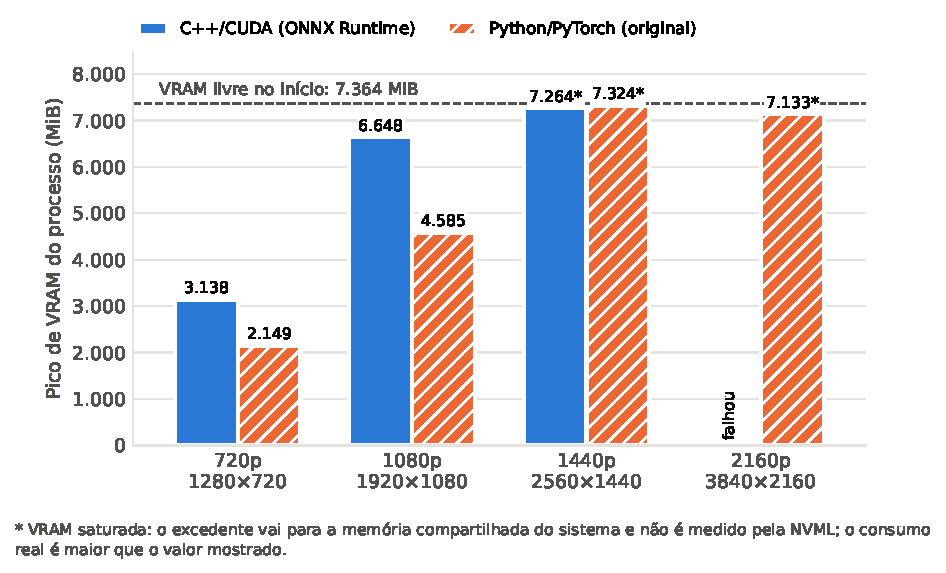
\includegraphics[width=\linewidth,height=6cm,keepaspectratio]{imagens/vram.pdf}
    \end{column}
    \begin{column}{0.36\textwidth}
      \small
      \begin{itemize}
        \item Contrário à hipótese: \destaque{cerca de 45\% a mais} de VRAM.
        \item 1080p: 6.648 MiB contra 4.585 MiB.
        \item H2 não atendido.
        \item Trocar de linguagem, sozinho, não reduz a memória.
      \end{itemize}
    \end{column}
  \end{columns}
\end{frame}

\begin{frame}{v2: memória limitada pelo bloco}
  \begin{columns}[T]
    \begin{column}{0.5\textwidth}
      \centering
      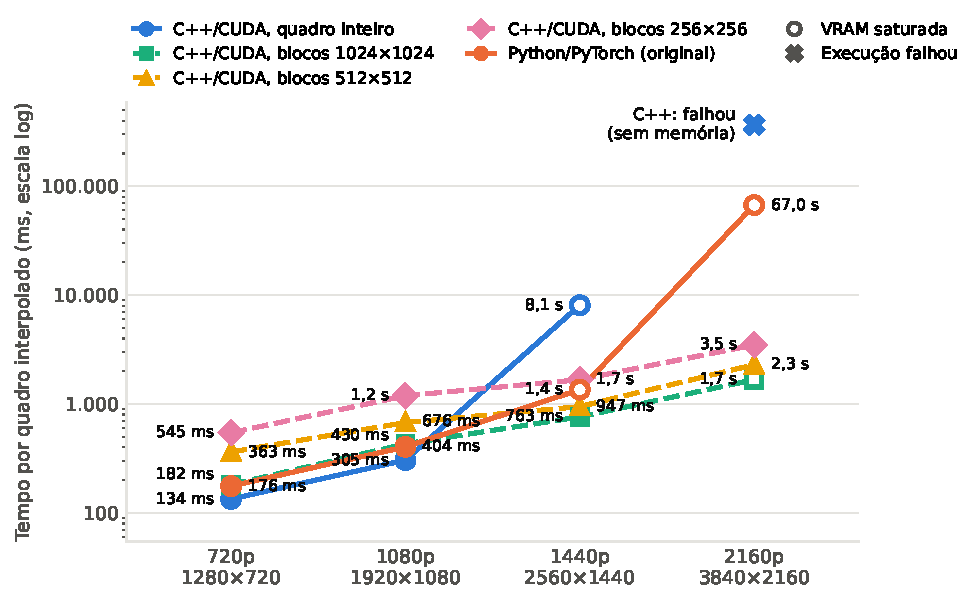
\includegraphics[width=\linewidth,height=4.5cm,keepaspectratio]{imagens/latencia_blocos.pdf}
    \end{column}
    \begin{column}{0.5\textwidth}
      \centering
      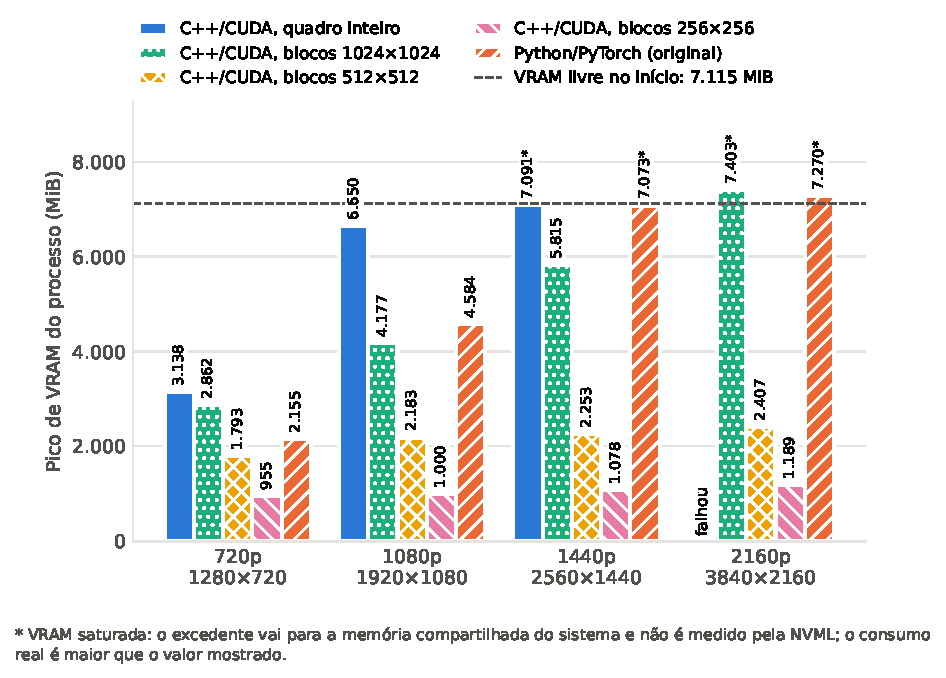
\includegraphics[width=\linewidth,height=4.5cm,keepaspectratio]{imagens/vram_blocos.pdf}
    \end{column}
  \end{columns}
  \vspace{2pt}
  \footnotesize
  \begin{itemize}
    \item Blocos de 512: de 1.793 MiB (720p) a 2.407 MiB (2160p); em 2160p, 2,3 s contra 67,0 s.
    \item Custo: a rede processa de 1,15 a 2,9 vezes a área do quadro. Em 720p e 1080p, nenhuma configuração atende H1 e H2 ao mesmo tempo.
  \end{itemize}
\end{frame}

\begin{frame}{v3: FP16 com o quadro inteiro}
  \begin{columns}[T]
    \begin{column}{0.48\textwidth}
      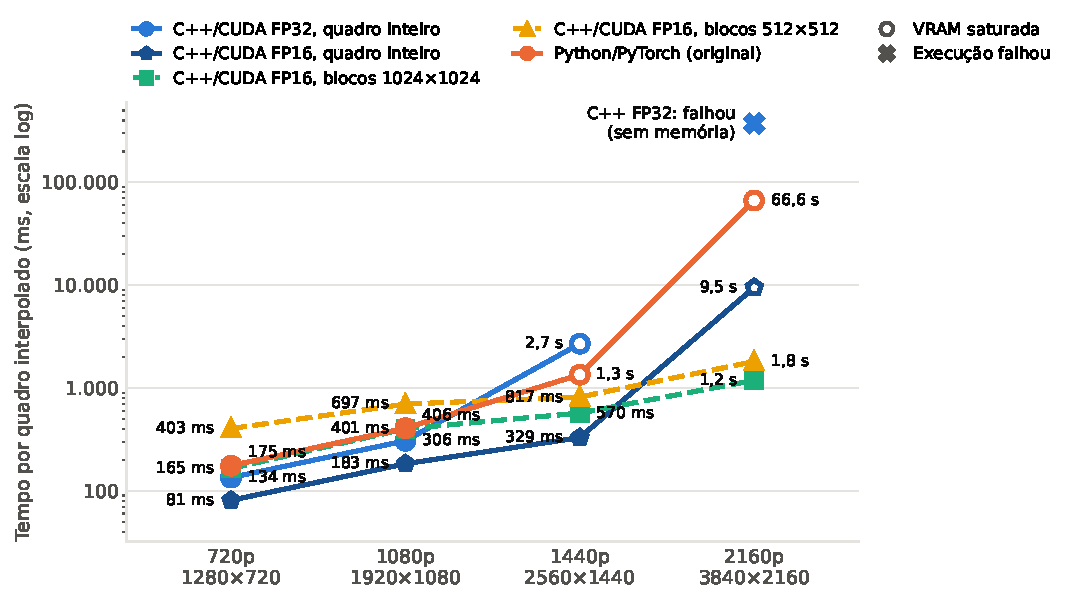
\includegraphics[width=\linewidth,height=5.2cm,keepaspectratio]{imagens/latencia_fp16.pdf}
    \end{column}
    \begin{column}{0.5\textwidth}
      \footnotesize
      \setlength{\tabcolsep}{3pt}
      \begin{tabular}{lrrrr}
        \toprule
         & \multicolumn{2}{c}{\textbf{Motor FP16}} & \multicolumn{2}{c}{\textbf{Original}} \\
        \textbf{Res.} & \textbf{ms} & \textbf{MiB} & \textbf{ms} & \textbf{MiB} \\
        \midrule
        720p & 80,8 & 1.554 & 175,3 & 2.149 \\
        1080p & 183,0 & 3.049 & 406,3 & 4.582 \\
        1440p & 329,0 & 4.800 & 1.345,8$^{*}$ & 7.204$^{*}$ \\
        \bottomrule
      \end{tabular}
      \nota{$^{*}$ VRAM saturada.}
      \vspace{4pt}
      \begin{itemize}
        \item 1080p: \destaque{$-55\%$ de tempo e 67\% da VRAM}.
        \item 1440p agora cabe, 4,1 vezes mais rápido.
        \item 2160p, FP16 com blocos de 1024: 1,19 s e 3.061 MiB, contra 66,6 s da original.
      \end{itemize}
    \end{column}
  \end{columns}
\end{frame}

\begin{frame}{As quatro combinações}
  \centering
  \footnotesize
  \setlength{\tabcolsep}{4pt}
  \begin{tabular}{lrrrrrrrr}
    \toprule
     & \multicolumn{2}{c}{\textbf{Python FP32}} & \multicolumn{2}{c}{\textbf{Python FP16}} & \multicolumn{2}{c}{\textbf{C++ FP32}} & \multicolumn{2}{c}{\textbf{C++ FP16}} \\
    \textbf{Res.} & \textbf{ms} & \textbf{MiB} & \textbf{ms} & \textbf{MiB} & \textbf{ms} & \textbf{MiB} & \textbf{ms} & \textbf{MiB} \\
    \midrule
    720p & 176,0 & 2.146 & 132,3 & 1.837 & 133,6 & 2.940 & 80,2 & 1.555 \\
    1080p & 405,5 & 4.585 & 303,9 & 3.801 & 306,0 & 4.888 & 183,0 & 3.057 \\
    1440p & 1.343,7$^{*}$ & 6.721$^{*}$ & 543,6 & 6.583 & 2.635,3$^{*}$ & 7.231$^{*}$ & 329,0 & 4.771 \\
    \bottomrule
  \end{tabular}
  \nota{$^{*}$ VRAM saturada. O C++ FP32 em 1440p atingiu 96,5\% da capacidade, abaixo do limiar de 97\%, e foi tratado como saturado pelo tempo.}
  \vspace{8pt}
  \raggedright\small
  \begin{itemize}
    \item Comparar C++ em FP16 com Python em FP32 mistura dois efeitos.
    \item A original roda em FP16 com \texttt{torch.autocast}, sem alterar o código.
    \item Em FP16, o PyTorch alcança o motor em FP32: 303,9 ms contra 306,0 ms em 1080p.
  \end{itemize}
\end{frame}

\begin{frame}{De onde vem cada ganho}
  \centering
  \small
  \begin{tabular}{lcccc}
    \toprule
     & \multicolumn{2}{c}{\textbf{Latência}} & \multicolumn{2}{c}{\textbf{VRAM (fração)}} \\
    \textbf{Comparação} & \textbf{720p} & \textbf{1080p} & \textbf{720p} & \textbf{1080p} \\
    \midrule
    C++ $\times$ Python, em FP32 & $-24{,}1\%$ & $-24{,}6\%$ & 137\% & 107\% \\
    C++ $\times$ Python, em FP16 & $-39{,}4\%$ & $-39{,}8\%$ & 85\% & 80\% \\
    \midrule
    FP16 $\times$ FP32, no Python & $-24{,}8\%$ & $-25{,}1\%$ & 86\% & 83\% \\
    FP16 $\times$ FP32, no C++ & $-40{,}0\%$ & $-40{,}2\%$ & 53\% & 63\% \\
    \midrule
    \rowcolor{senacblue!15}
    \textbf{C++ FP16 $\times$ Python FP32} & $\mathbf{-54{,}4\%}$ & $\mathbf{-54{,}9\%}$ & \textbf{72\%} & \textbf{67\%} \\
    \bottomrule
  \end{tabular}
  \nota{Todas as reduções de latência têm $p < 0{,}001$. VRAM: pico do primeiro termo como fração do pico do segundo.}
  \vspace{4pt}
  \raggedright\small
  \begin{itemize}
    \item \textbf{Os dois fatores contam}, e nenhum explica sozinho os 55\%.
    \item \textbf{Memória:} em FP32 o motor gasta mais; em FP16, menos. Parte disso vem de manter os filtros em FP16 na síntese, parcela que não foi isolada.
  \end{itemize}
\end{frame}

\begin{frame}{Fidelidade visual}
  \begin{columns}[T]
    \begin{column}{0.46\textwidth}
      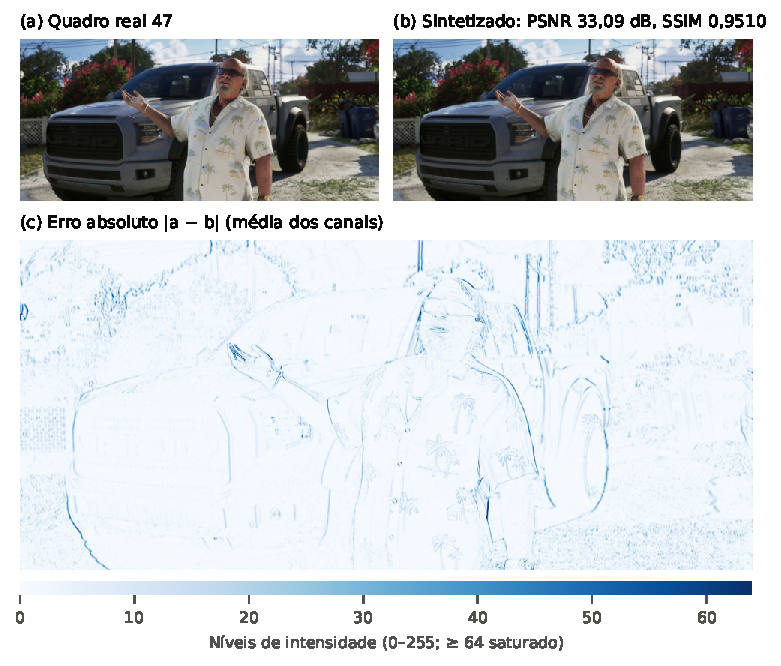
\includegraphics[width=\linewidth,height=5.4cm,keepaspectratio]{imagens/comparacao_quadro_1080p.pdf}
      \fontefig{elaborado pelo autor, com quadros do trailer (ROCKSTAR GAMES, 2025).}
    \end{column}
    \begin{column}{0.52\textwidth}
      \footnotesize
      \setlength{\tabcolsep}{3pt}
      \begin{tabular}{lcccc}
        \toprule
         & \multicolumn{2}{c}{\textbf{PSNR (dB)}} & \multicolumn{2}{c}{\textbf{SSIM}} \\
         & \textbf{Midd.} & \textbf{Vimeo} & \textbf{Midd.} & \textbf{Vimeo} \\
        \midrule
        C++ FP32 & 37,22 & 34,46 & 0,9680 & 0,9590 \\
        C++ FP16 & 37,22 & 34,46 & 0,9679 & 0,9590 \\
        Python & 37,22 & 34,46 & 0,9680 & 0,9590 \\
        \bottomrule
      \end{tabular}
      \vspace{6pt}
      \begin{itemize}
        \item Vídeo em 1080p: 34,10 dB, SSIM 0,9538 e VMAF 77,4 nas duas implementações.
        \item H3 atendido em todas as versões.
        \item O erro se concentra nas bordas de objetos em movimento.
        \item A forma de execução não muda a qualidade.
      \end{itemize}
    \end{column}
  \end{columns}
\end{frame}

\begin{frame}{Análise frente à hipótese (720p / 1080p)}
  \centering
  \small
  \renewcommand{\arraystretch}{1.2}
  \begin{tabular}{llccc}
    \toprule
    \textbf{Versão} & \textbf{Configuração} & \textbf{Latência} & \textbf{VRAM} & \textbf{H1 e H2} \\
    \midrule
    v1 & FP32, quadro inteiro & $-24{,}3\%$ / $-24{,}6\%$ & $+46\%$ / $+45\%$ & só H1 \\
    v2 & FP32, blocos 512 & $+106\%$ / $+67\%$ & 83\% / 48\% & só H2 \\
    v3 & FP32, quadro inteiro & $-23{,}3\%$ / $-24{,}6\%$ & 137\% / 107\% & só H1 \\
    \rowcolor{senacblue!15}
    \textbf{v3} & \textbf{FP16, quadro inteiro} & $\mathbf{-53{,}9\%}$ / $\mathbf{-55{,}0\%}$ & \textbf{72\% / 67\%} & \textbf{H1 e H2} \\
    v3 & FP16, blocos 1024 & $-6{,}0\%$ / $-1{,}3\%$ & 73\% / 62\% & só H2 \\
    \bottomrule
  \end{tabular}
  \nota{Em relação à original em FP32. Na v1, a VRAM é a variação do pico; nas demais, a fração do pico da original.}
  \vspace{6pt}
  \raggedright\small
  \begin{itemize}
    \item H3 foi atendido em todas as configurações.
    \item Contra a original também em FP16, o motor em FP16 ainda atende H1 e H2: $-39{,}8\%$ e 80\% em 1080p.
  \end{itemize}
\end{frame}

% ===============================================================
\section{Conclusão}
% ===============================================================
\begin{frame}{Resposta à pergunta de pesquisa}
  \begin{block}{Afirmativa, com uma ressalva sobre a origem de cada ganho}
    Em 1080p, o motor em FP16 levou 183,0 ms contra 406,3 ms, com 67\% da VRAM e a mesma qualidade.
  \end{block}
  \vspace{4pt}
  \small
  \begin{itemize}
    \item \textbf{Latência:} vem da forma de execução, presente desde a v1, e é ampliada pela precisão numérica.
    \item \textbf{Memória:} não vem da troca de linguagem. Vem de decisões explícitas sobre o alocador, a precisão e, quando necessário, o processamento em blocos.
    \item O motor nativo torna essas decisões diretamente controláveis.
  \end{itemize}
\end{frame}

\begin{frame}{Contribuições}
  \small
  \begin{enumerate}
    \item Constatação medida: trocar linguagem e \textit{framework} reduz a latência, mas não reduz por si só a memória;
    \item Separação do efeito da forma de execução e do efeito da precisão, pelas quatro combinações;
    \item Identificação do padrão de memória do ONNX Runtime como principal fonte do excedente;
    \item Quantificação do compromisso entre memória e latência no processamento em blocos;
    \item Meia precisão com filtros em FP16 e acumulação em FP32, sem perda de fidelidade;
    \item Protocolo de testes reprodutível, que considera o \textit{Sysmem Fallback} do Windows;
    \item Motor verificado contra a original e exportação ONNX corrigida.
  \end{enumerate}
\end{frame}

\begin{frame}{Limitações e trabalhos futuros}
  \footnotesize
  \begin{columns}[T]
    \begin{column}{0.5\textwidth}
      \textbf{Limitações}
      \begin{itemize}
        \item Desempenho medido em um único trecho de 61 quadros, sem fixar os \textit{clocks}.
        \item Em 2160p, só 3 medições e 4 quadros avaliados.
        \item Python em FP16 só pelo \texttt{autocast}.
        \item Vimeo-90K: 200 trios, de uma cópia pública.
        \item Condição de controle não executada; original medida só pelo tempo total.
        \item O limiar de 97\% deixou de sinalizar uma saturação.
      \end{itemize}
    \end{column}
    \begin{column}{0.5\textwidth}
      \textbf{Trabalhos futuros}
      \begin{itemize}
        \item Reduzir o custo dos blocos: tamanho automático, formato fixo e margens menores.
        \item Explicar por que o FP16 acelera mais o motor que o PyTorch, medindo por estágio.
        \item Comparar com TensorRT e quantização em 8 bits.
        \item Executar a condição de controle.
        \item Ampliar a base: mais vídeos, Vimeo-90K completo e repetições das baterias.
      \end{itemize}
    \end{column}
  \end{columns}
\end{frame}

\begin{frame}[plain]
  \centering
  \vspace{0.8cm}
  \logosenacgrande

  \vspace{0.7cm}
  {\Large\bfseries\color{senacblue}Obrigado!\par}
  \vspace{0.3cm}
  {\normalsize Perguntas?\par}
  \vspace{0.5cm}
  {\footnotesize Pedro Henrique Gomes\par}
\end{frame}

% ===============================================================
% APÊNDICE (slides de apoio para a arguição da banca)
% ===============================================================
\appendix

\begin{frame}{Apoio: o que é FP16}
  \centering
  \small
  \renewcommand{\arraystretch}{1.2}
  \begin{tabular}{lcc}
    \toprule
     & \textbf{FP32} & \textbf{FP16} \\
    \midrule
    Bits por número & 32 & 16 \\
    Dígitos de precisão, aproximados & 7 & 3 \\
    Maior valor representável & $\approx 3{,}4 \times 10^{38}$ & 65.504 \\
    Menor passo perto de 1 & $\approx 1{,}2 \times 10^{-7}$ & $\approx 0{,}00098$ \\
    \bottomrule
  \end{tabular}
  \vspace{8pt}
  \raggedright
  \begin{itemize}
    \item Em FP16, $1 + 0{,}0004 = 1$: o termo pequeno some.
    \item Por isso, média, desvio padrão e acumulação da síntese seguem em FP32.
    \item A rede e os filtros ficam em FP16.
  \end{itemize}
\end{frame}

\begin{frame}{Apoio: ambiente experimental}
  \centering
  \footnotesize
  \renewcommand{\arraystretch}{1.15}
  \begin{tabular}{lp{10.3cm}}
    \toprule
    \textbf{Componente} & \textbf{Especificação} \\
    \midrule
    GPU & NVIDIA GeForce RTX 4060 Ti, 8 GB de VRAM \\
    CPU e memória & Intel Core i5-12400F, 16 GB \\
    Sistema & Windows 11 Home; \textit{driver} 610.47 na 1ª bateria e 610.88 nas demais \\
    Motor C++ & C++17, CUDA Toolkit 13.3, MSVC (Visual Studio 2022), CMake 4.4 \\
    Inferência & ONNX Runtime 1.23.2 com \textit{CUDA Execution Provider} \\
    Vídeo & OpenCV 4.13 \\
    Original & Python 3.10, PyTorch 2.11 (CUDA 12.8) \\
    Métricas & scikit-image 0.25 (PSNR e SSIM), FFmpeg 9.0 com \textit{libvmaf} \\
    \bottomrule
  \end{tabular}
\end{frame}

\begin{frame}{Apoio: resultados da v1}
  \centering
  \scriptsize
  \setlength{\tabcolsep}{3pt}
  \begin{tabular}{llrrrrrr}
    \toprule
    \textbf{Res.} & \textbf{Implementação} & \textbf{ms/quadro} & \textbf{FPS} & \textbf{VRAM (MiB)} & \textbf{PSNR (dB)} & \textbf{SSIM} & \textbf{VMAF} \\
    \midrule
    720p & C++/CUDA & 133,9 $\pm$ 0,4 & 7,47 & 3.138 & 34,48 & 0,9622 & 85,16 \\
    720p & Python/PyTorch & 176,8 $\pm$ 1,0 & 5,65 & 2.149 & 34,48 & 0,9622 & 85,16 \\
    \midrule
    1080p & C++/CUDA & 305,5 $\pm$ 1,8 & 3,27 & 6.648 & 34,10 & 0,9538 & 77,42 \\
    1080p & Python/PyTorch & 404,9 $\pm$ 2,2 & 2,47 & 4.585 & 34,10 & 0,9538 & 77,42 \\
    \midrule
    1440p & C++/CUDA & 7.745,1 $\pm$ 214,5$^{*}$ & 0,13 & 7.264$^{*}$ & 34,04 & 0,9532 & 71,91 \\
    1440p & Python/PyTorch & 1.344,5 $\pm$ 3,8$^{*}$ & 0,74 & 7.324$^{*}$ & 34,04 & 0,9532 & 71,91 \\
    \midrule
    2160p & C++/CUDA & \multicolumn{6}{c}{falhou por falta de memória} \\
    2160p & Python/PyTorch & 64.900,5 $\pm$ 3.452,8$^{*}$ & 0,02 & 7.133$^{*}$ & 31,44 & 0,9323 & 50,33 \\
    \bottomrule
  \end{tabular}
  \nota{$^{*}$ VRAM saturada: o excedente vai para a memória principal e não é contabilizado pela NVML.}
\end{frame}

\begin{frame}{Apoio: resultados da v2}
  \centering
  \tiny
  \renewcommand{\arraystretch}{0.92}
  \begin{tabular}{llrrr}
    \toprule
    \textbf{Res.} & \textbf{Implementação} & \textbf{ms/quadro} & \textbf{FPS} & \textbf{VRAM (MiB)} \\
    \midrule
    720p & C++/CUDA, quadro inteiro & 134,1 $\pm$ 0,8 & 7,46 & 3.138 \\
    720p & C++/CUDA, blocos 1024 & 181,6 $\pm$ 8,0 & 5,51 & 2.862 \\
    720p & C++/CUDA, blocos 512 & 362,5 $\pm$ 19,2 & 2,76 & 1.793 \\
    720p & C++/CUDA, blocos 256 & 545,1 $\pm$ 24,4 & 1,83 & 955 \\
    720p & Python/PyTorch & 176,2 $\pm$ 0,9 & 5,68 & 2.155 \\
    \midrule
    1080p & C++/CUDA, quadro inteiro & 305,3 $\pm$ 1,8 & 3,28 & 6.650 \\
    1080p & C++/CUDA, blocos 1024 & 430,5 $\pm$ 5,4 & 2,32 & 4.177 \\
    1080p & C++/CUDA, blocos 512 & 676,0 $\pm$ 11,7 & 1,48 & 2.183 \\
    1080p & C++/CUDA, blocos 256 & 1.190,4 $\pm$ 29,3 & 0,84 & 1.000 \\
    1080p & Python/PyTorch & 404,2 $\pm$ 1,8 & 2,47 & 4.584 \\
    \midrule
    1440p & C++/CUDA, quadro inteiro & 8.074,8 $\pm$ 10,8$^{*}$ & 0,12 & 7.091$^{*}$ \\
    1440p & C++/CUDA, blocos 1024 & 762,7 $\pm$ 16,0 & 1,31 & 5.815 \\
    1440p & C++/CUDA, blocos 512 & 947,4 $\pm$ 10,3 & 1,06 & 2.253 \\
    1440p & C++/CUDA, blocos 256 & 1.673,7 $\pm$ 49,0 & 0,60 & 1.078 \\
    1440p & Python/PyTorch & 1.354,7 $\pm$ 10,9$^{*}$ & 0,74 & 7.073$^{*}$ \\
    \midrule
    2160p & C++/CUDA, quadro inteiro & \multicolumn{3}{c}{falhou por falta de memória} \\
    2160p & C++/CUDA, blocos 1024 & 1.673,2 $\pm$ 5,0$^{*}$ & 0,60 & 7.403$^{*}$ \\
    2160p & C++/CUDA, blocos 512 & 2.296,4 $\pm$ 5,6 & 0,44 & 2.407 \\
    2160p & C++/CUDA, blocos 256 & 3.490,0 $\pm$ 5,6 & 0,29 & 1.189 \\
    2160p & Python/PyTorch & 67.031,9 $\pm$ 2.189,8$^{*}$ & 0,01 & 7.270$^{*}$ \\
    \bottomrule
  \end{tabular}
\end{frame}

\begin{frame}{Apoio: resultados da v3}
  \centering
  \tiny
  \renewcommand{\arraystretch}{0.92}
  \begin{tabular}{llrrr}
    \toprule
    \textbf{Res.} & \textbf{Implementação} & \textbf{ms/quadro} & \textbf{FPS} & \textbf{VRAM (MiB)} \\
    \midrule
    720p & C++/CUDA FP32, quadro inteiro & 134,4 $\pm$ 0,9 & 7,44 & 2.944 \\
    720p & C++/CUDA FP16, quadro inteiro & 80,8 $\pm$ 0,9 & 12,38 & 1.554 \\
    720p & C++/CUDA FP16, blocos 1024 & 164,7 $\pm$ 5,6 & 6,07 & 1.568 \\
    720p & C++/CUDA FP16, blocos 512 & 403,0 $\pm$ 11,5 & 2,48 & 893 \\
    720p & Python/PyTorch & 175,3 $\pm$ 0,8 & 5,70 & 2.149 \\
    \midrule
    1080p & C++/CUDA FP32, quadro inteiro & 306,2 $\pm$ 1,2 & 3,27 & 4.887 \\
    1080p & C++/CUDA FP16, quadro inteiro & 183,0 $\pm$ 0,6 & 5,46 & 3.049 \\
    1080p & C++/CUDA FP16, blocos 1024 & 401,0 $\pm$ 24,9 & 2,49 & 2.855 \\
    1080p & C++/CUDA FP16, blocos 512 & 696,8 $\pm$ 37,3 & 1,44 & 920 \\
    1080p & Python/PyTorch & 406,3 $\pm$ 1,7 & 2,46 & 4.582 \\
    \midrule
    1440p & C++/CUDA FP32, quadro inteiro & 2.694,7 $\pm$ 9,7$^{*}$ & 0,37 & 7.149$^{*}$ \\
    1440p & C++/CUDA FP16, quadro inteiro & 329,0 $\pm$ 0,8 & 3,04 & 4.800 \\
    1440p & C++/CUDA FP16, blocos 1024 & 570,3 $\pm$ 5,0 & 1,75 & 2.915 \\
    1440p & C++/CUDA FP16, blocos 512 & 816,7 $\pm$ 8,9 & 1,22 & 979 \\
    1440p & Python/PyTorch & 1.345,8 $\pm$ 3,7$^{*}$ & 0,74 & 7.204$^{*}$ \\
    \midrule
    2160p & C++/CUDA FP32, quadro inteiro & \multicolumn{3}{c}{falhou por falta de memória} \\
    2160p & C++/CUDA FP16, quadro inteiro & 9.502,7 $\pm$ 43,8$^{*}$ & 0,11 & 7.370$^{*}$ \\
    2160p & C++/CUDA FP16, blocos 1024 & 1.187,7 $\pm$ 2,2 & 0,84 & 3.061 \\
    2160p & C++/CUDA FP16, blocos 512 & 1.808,1 $\pm$ 12,7 & 0,55 & 1.127 \\
    2160p & Python/PyTorch & 66.594,4 $\pm$ 1.768,6$^{*}$ & 0,02 & 7.357$^{*}$ \\
    \bottomrule
  \end{tabular}
\end{frame}

\begin{frame}{Apoio: estágios e PSNR por quadro}
  \begin{columns}[T]
    \begin{column}{0.5\textwidth}
      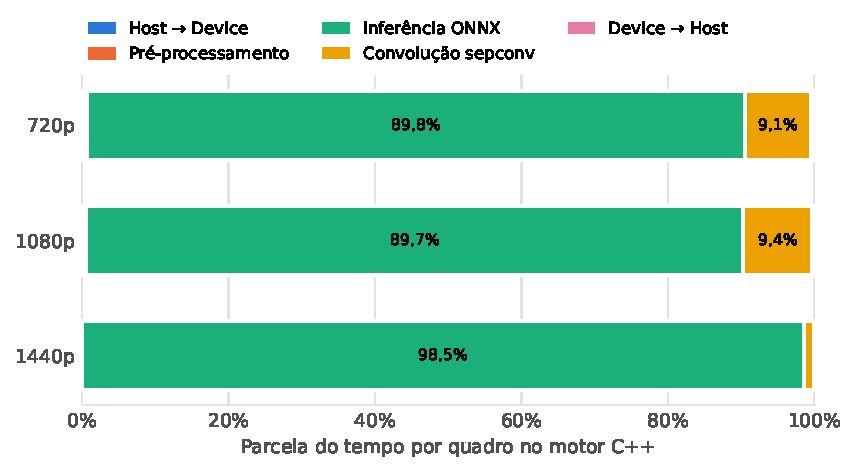
\includegraphics[width=\linewidth]{imagens/etapas_cpp.pdf}
      \nota{A inferência responde por cerca de 90\% do tempo em 1080p; as transferências e o pré-processamento somam menos de 1\%.}
    \end{column}
    \begin{column}{0.5\textwidth}
      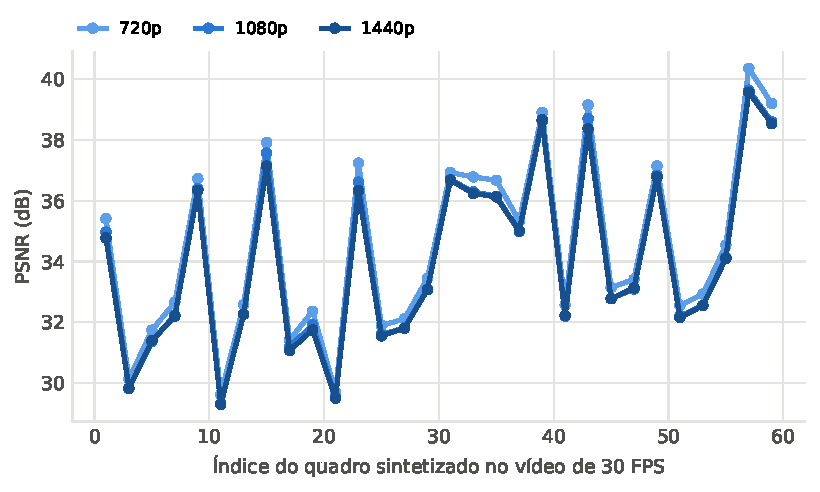
\includegraphics[width=\linewidth]{imagens/psnr_quadros.pdf}
      \nota{As curvas têm o mesmo formato nas três resoluções: a dificuldade depende do conteúdo de cada instante.}
    \end{column}
  \end{columns}
\end{frame}

\begin{frame}{Apoio: fluxo óptico (RAFT)}
  \centering
  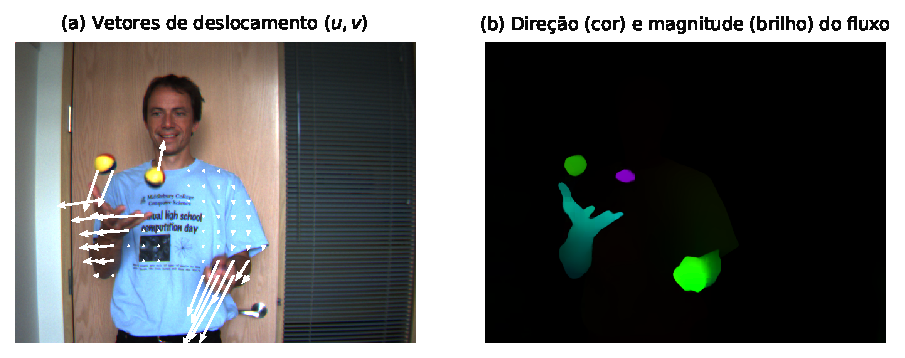
\includegraphics[width=\textwidth]{imagens/fluxo_optico.pdf}
  \fontefig{elaborado pelo autor, com o RAFT da biblioteca torchvision e a sequência Beanbags (BAKER et al., 2011).}
  \vspace{4pt}
  \raggedright\small
  \begin{itemize}
    \item Usado só nesta ilustração: não faz parte do motor nem das medições.
    \item Bola central: RAFT, cerca de $(+7,-35)$ pixels; filtros do SepConv++, cerca de $(+4,-30)$.
  \end{itemize}
\end{frame}

\begin{frame}{Apoio: execução paralela na GPU (SIMT)}
  \centering
  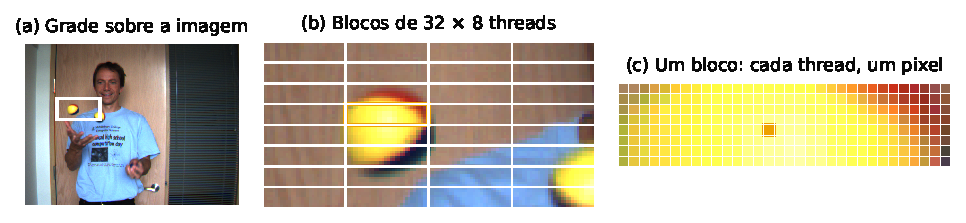
\includegraphics[width=\textwidth]{imagens/simt.pdf}
  \fontefig{elaborado pelo autor, com a sequência Beanbags (BAKER et al., 2011).}
  \vspace{4pt}
  \raggedright\small
  \begin{itemize}
    \item Uma grade de blocos cobre a imagem; cada bloco tem $32 \times 8$ \textit{threads}.
    \item Cada \textit{thread} calcula um pixel.
  \end{itemize}
\end{frame}

\begin{frame}{Apoio: por que usar mais de uma métrica}
  \centering
  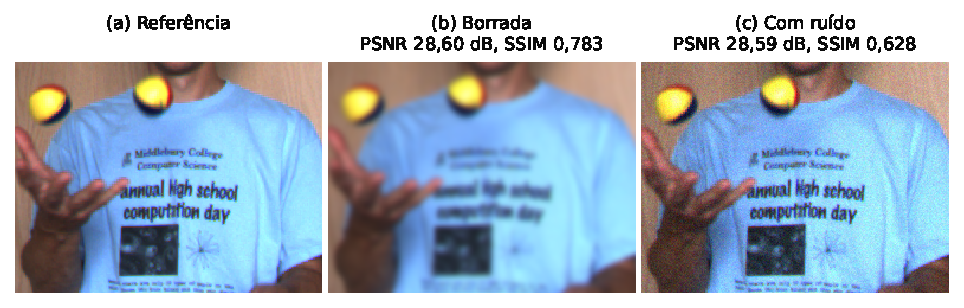
\includegraphics[width=\textwidth]{imagens/metricas.pdf}
  \fontefig{elaborado pelo autor, com a sequência Beanbags (BAKER et al., 2011).}
  \vspace{4pt}
  \raggedright\small
  \begin{itemize}
    \item Mesmo PSNR, cerca de 28,6 dB, e SSIM diferente: 0,783 e 0,628.
    \item O VMAF acrescenta uma avaliação perceptual, voltada a vídeo.
  \end{itemize}
\end{frame}

\begin{frame}{Apoio: escolha da margem (1080p)}
  \centering
  \small
  \begin{tabular}{rrrrr}
    \toprule
    \textbf{Bloco} & \textbf{Margem} & \textbf{PSNR (dB)} & \textbf{Dif. máx.} & \textbf{ms/quadro} \\
    \midrule
    512 & 0 & 57,48 & 63 & 382 \\
    512 & 64 & 81,26 & 2 & 496 \\
    \rowcolor{senacblue!15}
    \textbf{512} & \textbf{96} & \textbf{98,36} & \textbf{1} & \textbf{570} \\
    512 & 160 & 104,61 & 1 & 747 \\
    \midrule
    256 & 0 & 53,34 & 98 & 431 \\
    256 & 96 & 95,17 & 1 & 820 \\
    \bottomrule
  \end{tabular}
  \nota{PSNR e diferença máxima em relação ao quadro inteiro, na reimplementação em PyTorch, em três pares de quadros.}
\end{frame}

\begin{frame}[fragile]{Apoio: trecho do \textit{kernel} de síntese}
\tiny
\begin{verbatim}
__device__ float accumulate_frame(const float* frame, const Filter* ver,
                                  const Filter* hor, ..., int x, int y, float acc[3])
{
    constexpr int R = K / 2;               // raio = 25
    float h[K]; int sx[K]; float hor_sum = 0.0f;

    for (int fx = 0; fx < K; ++fx) {       // le o filtro horizontal uma vez
        h[fx]  = to_float(hor[fx * filter_plane + filter_pixel]);
        sx[fx] = min(max(x + fx - R, 0), width - 1);   // borda replicada
        hor_sum += h[fx];
    }

    float ver_sum = 0.0f;
    for (int fy = 0; fy < K; ++fy) {       // para cada linha da vizinhanca
        const float v = to_float(ver[fy * filter_plane + filter_pixel]);
        ver_sum += v;
        const int sy = min(max(y + fy - R, 0), height - 1);
        const float* row = frame + (size_t)sy * width;

        float row_b = 0, row_g = 0, row_r = 0;
        for (int fx = 0; fx < K; ++fx) {   // convolucao horizontal da linha
            row_b += h[fx] * row[sx[fx]];
            row_g += h[fx] * row[plane + sx[fx]];
            // ... idem para o canal R; depois, acumula com o peso v
\end{verbatim}
\normalsize
\vspace{-4pt}
Os dois laços aninhados mostram as $N^2$ multiplicações por pixel: a separabilidade reduz a memória, não as contas.
\end{frame}

\end{document}
